%%%%%%%%%%%%%%%%%%%%%%%%%%%%%%%%%%%%%%%%%%%%%%%%%%%
%% LaTeX book template                           %%
%% Author:  Amber Jain (http://amberj.devio.us/) %%
%% License: ISC license                          %%
%%%%%%%%%%%%%%%%%%%%%%%%%%%%%%%%%%%%%%%%%%%%%%%%%%%

\documentclass[a4paper,11pt, oneside]{book}
\usepackage[T1]{fontenc}
\usepackage[utf8]{inputenc}
\usepackage{lmodern}
\usepackage{mathptmx}

% Uncomment to set page margin to 2.5 cm.
%\usepackage[margin=2.5cm]{geometry}

%%%%%%%%%%%%%%%%%%%%%%%%%%%%%%%%%%%%%%%%%%%%%%%%%%%%%%%%%
% Source: http://en.wikibooks.org/wiki/LaTeX/Hyperlinks %
%%%%%%%%%%%%%%%%%%%%%%%%%%%%%%%%%%%%%%%%%%%%%%%%%%%%%%%%%
\usepackage{hyperref}
\hypersetup{
	colorlinks=true,
	linkcolor=blue,
	filecolor=magenta,      
	urlcolor=cyan,
	citecolor=gray,
}
\usepackage{graphicx}
\usepackage[english]{babel}
\usepackage{verbatimbox}
\usepackage{graphicx}
\graphicspath{ {schedule/}{diagrams/}{graphs/} }
\usepackage{float}
\usepackage{pdfpages}

%%%%%%%%%%%%%%%%%%%%%%%%%%%%%%%%%%%%%%%%%%%%%%%%%%%%%%%%%%%%%%%%%%%%%%%%%%%%%%%%
% 'dedication' environment: To add a dedication paragraph at the start of book %
% Source: http://www.tug.org/pipermail/texhax/2010-June/015184.html            %
%%%%%%%%%%%%%%%%%%%%%%%%%%%%%%%%%%%%%%%%%%%%%%%%%%%%%%%%%%%%%%%%%%%%%%%%%%%%%%%%
\newenvironment{dedication}
{
   \cleardoublepage
   \thispagestyle{empty}
   \vspace*{\stretch{1}}
   \hfill\begin{minipage}[t]{0.66\textwidth}
   \raggedright
}
{
   \end{minipage}
   \vspace*{\stretch{3}}
   \clearpage
}

%%%%%%%%%%%%%%%%%%%%%%%%%%%%%%%%%%%%%%%%%%%%%%%%
% Chapter quote at the start of chapter        %
% Source: http://tex.stackexchange.com/a/53380 %
%%%%%%%%%%%%%%%%%%%%%%%%%%%%%%%%%%%%%%%%%%%%%%%%
\makeatletter
\renewcommand{\@chapapp}{}% Not necessary...
\newenvironment{chapquote}[2][2em]
  {\setlength{\@tempdima}{#1}%
   \def\chapquote@author{#2}%
   \parshape 1 \@tempdima \dimexpr\textwidth-2\@tempdima\relax%
   \itshape}
  {\par\normalfont\hfill--\ \chapquote@author\hspace*{\@tempdima}\par\bigskip}
\makeatother

%%%%%%%%%%%%%%%%%%%%%%%%%%%%%%%%%%%%%%%%%%%%%%%%%%%
% First page of book which contains 'stuff' like: %
%  - Book title, subtitle                         %
%  - Book author name                             %
%%%%%%%%%%%%%%%%%%%%%%%%%%%%%%%%%%%%%%%%%%%%%%%%%%%

% Book's title and subtitle
\title{\Huge \textbf{Road Surface Estimator} \\ \huge Final Report}
% Author
\author{
	\textsc{Thanakrit Lee}
	\\
	26529009
	\\
	tlee38@student.monash.edu
	\\
	Monash University
}

\begin{document}
	
\frontmatter
\maketitle

%%%%%%%%%%%%%%%%%%%%%%%%%%%%%%%%%%%%%%%%%%%%%%%%%%%%%%%%%%%%%%%%%%%%%%%%

\begin{center}
	\textbf{Abstract}
\end{center}
The purpose of the project is to develop an application that estimate the total surface area of a 1 square $km^2$ area on the map. There are many different ways to go about implementing a solution. Neural Networks could be use to find roads in a map image, but in this project a simpler solution is implemented. 
\\\\
A server is use to do the surface area calculation by extracting road pixels from an image of the map. The calculation result is send to the application front end client, featuring an elegant and responsive display of user interface to work with. A separation of client and server is implemented so that heavy calculation processing work can be done remotely, faster, more efficient, and doesn't rely on the performance of the user device.

\begin{center}
	\textbf{Keywords}
\end{center}
\begin{center}
	Road, surface area, latitude, longitude, google maps
\end{center}

\begin{center}
	\textbf{Word Count}
\end{center}
\begin{center}
	5405 words
\end{center}




%%%%%%%%%%%%%%%%%%%%%%%%%%%%%%%%%%%%%%%%%%%%%%%%%%%%%%%%%%%%%%%%%%%%%%%%
% Auto-generated table of contents, list of figures and list of tables %
%%%%%%%%%%%%%%%%%%%%%%%%%%%%%%%%%%%%%%%%%%%%%%%%%%%%%%%%%%%%%%%%%%%%%%%%
\tableofcontents

\mainmatter

%%%%%%%%%%%%%%%%%%%%%%%%%%%%%%%%%%%%%%%%%%%%%%%%%%%%%%%%%%%%%%%%%%%%%%%%

\chapter{Introduction}

Re-surfacing roads requires the knowledge of the surface area of roads to resurface.
Getting the surface area of roads can be made more efficient using aerial/satellite views technology, where the surface area can be calculated. The efficiency of having a total estimated surface area of roads to resurface allows road surface materials to be prepared in a more precise manner, reducing materials wastes and thus reducing total road resurfacing costs.

\section{Objective}

The objective of this application is to allow user to select a point on the map and to work out the total area of roads in the nominated square kilometre, where the specified point is the centre, to give a quote of the road resurfacing cost \cite{DOCUMENT_PROJECT_INTRO:1}.
\\\\
The web application allows user to designate point on a map for a total estimated surface area of roads in the square kilometre ($km^2$). The web application will be implemented with Google Maps, which allows for user-to-map interactivity, and for getting data requires for the surface area calculation.

\section{Requirements}

\subsection{Functional Requirements}

\begin{itemize}
	\item The application is able to display a graphical map.
	\item The application allow user to interact with the map e.g. click on the map, drag and move around on the map, zoom in and zoom out, change map styling (roadmap and satellite view), add marker, move marker by dragging it, click on marker to show marker info.
	\item The application allow user to mark the centre point of the square kilometre area on the interactive map.
	\item The application allow user to input longitude and latitude coordinates.
	\item The application is able to display the user input coordinates on the interactive map.
	\item The application is able to calculate the surface area of the road in the selected square kilometre ($km^2$).
	\item The application is able to display the calculated road surface area.
\end{itemize}

\subsection{Non-Functional Requirements}
\begin{itemize}
	\item The application's graphical user interface is easy to navigate.
	\item The application is doesn't take long to process the surface area calculation, i.e. low response time.
	\item The application is responsive.
	\item The application is able to be use on mobile devices.
	\item The application provides an easy to understand tutorial on how to use the application.
	\item The application is hosted on the web, and user can access via the internet.
\end{itemize}

\section{Constraints}

A constraint for the project is that this project is done as part of a contract for a local council in Victoria, Melbourne, Australia. This means that the roads to resurface must be the correct category of roads classified by the local council (i.e. the declared roads being free ways, arterial roads and some non-arterial state roads) \cite{WEBSITE_VICROAD:1}.


%%%%%%%%%%%%%%%%%%%%%%%%%%%%%%%%%%%%%%%%%%%%%%%%%%%%%%%%%%%%%%%%%%%%%%%%

\chapter{Background}

\section{Academic Literature Review}
\begin{itemize}
	\item FIT3036 Project Intro Document \cite{DOCUMENT_PROJECT_INTRO:1}.
	
	The document gives a brief introduction to what the project will be about and the main specifications for the project. This document was use as the main reference for getting the requirements for the project's application.
	
	
	\item The Google Maps JavaScript API Documentation \cite{WEBSITE_GOOGLE_MAPS:1}.
	
	The documentation pages was use to study the API and how to use it in the project. Google Maps API was chosen, because it was one of the recommended technologies to use in the project specified in the project intro document \cite{DOCUMENT_PROJECT_INTRO:1}.
	
	
	\item Road Detection Using Deep Neural Network In High Spatial Resolution Images \cite{ARTICLE_ROAD_DETECTION:1}.
	
	This was the first article I read about road detection. I initially had the idea that the road detection was going to be done using satellite images. This article provide me with an overall look idea of how road detection was done using satellite images and deep Convolutional Neural Network (CNN).
	
	Although in the end I didn't end up implementing the application using satellite images and neural network, this article gives me a perspective of the different ways the application could be implemented.
	
	
	\item A Medium \cite{WEBSITE_MEDIUM:1} article. Node.js get-pixels: Getting Pixels at Specific Sectors of an Image using ndarray \cite{WEBSITE_MEDIUM_NODEJS_GET-PIXELS:1}
	
	This Medium article is a tutorial describing the way to get each pixel of an image using Node.js \cite{WEBSITE_NODEJS:1} and the package: get-pixels \cite{WEBSITE_GET-PIXELS:1}. I use this article to understand how to get each pixel of the map image using get-pixels.
	
	The article was useful in that it is simple, to the point, and provide lots of usage examples, while the get-pixels documentation doesn't provide lots of example for me to understand its usage.
	
	I believe my lack of understanding using the get-pixels documentation was that it doesn't provide any examples for the image pixels data structure \cite{WEBSITE_NDARRAY:1}, while the Medium article does.
	
	
	\item Google Maps Static Api Documentation \cite{WEBSITE_GOOGLE_MAPS_STATIC:1}.
	
	This documentation was use to understand how to create a static image of Google map. The static image is needed so that it could be processed in the server to detect the road pixels. The documentation is simple to understand, since there isn't any new concept introduce. The map URL property is almost the same as the JavaScript API, but is converted into a static image instead.
	
	
	\item Angular 5 tutorial and documentation \cite{WEBSITE_ANGULAR:1}
	
	I've decided to use the Angular (5) framework, because I want to make my development process of the application easier. I've also decided to use Angular, because I've recently started learning the technology and wanted to implement my knowledge.
	
	The tutorial provide a basic concept and usage of the framework, but I've also use other sources such as YouTube videos and online tutorial.
	
	The documentation is easy to understand as long as one have a grasp of the previous pre-requisite concepts. 
	
	
	\item A YouTube video tutorial on Angular Google Maps (AGM). Google Maps \& Angular | ANGULAR SNIPPETS \cite{WEBSITE_YOUTUBE_AGM:1}.
	
	The video shows how to get AGM setup and goes through the basic usage of the package: showing the map on a html page, adding markers to the map, and centring the map on a latitude/longitude coordinates.
	
	
	\item A video and online tutorial on how to use material design \cite{WEBSITE_GOOGLE_MATERIAL_DESIGN:1} bootstrap \cite{WEBSITE_BOOTSTRAP:1} with angular by using the library MDBootstrap \cite{WEBSITE_MDBOOTSTRAP:1}. Material Design Bootstrap 4 and Angular 5 Tutorial - MdBootstrap \cite{WEBSITE_COURSETRO_MDBOOTSTRAP_ANGULAR:1}.
	
	
	\item Bootstrap 4 documentation \cite{WEBSITE_BOOTSTRAP:1}.
	
	The documentation is use for when I've encounter Bootstrap related problem and the MDBootstrap documentation isn't clear or have enough information.
	
	
	\item Google Maps APIs Styling Wizard \cite{WEBSITE_GOOGLE_MAPS_API_STYLING_WIZARD:1}.
	
	The styling wizard is a tool use for creating a style property of a Google Maps. The wizard shows options such as colours and visibility of elements on the map. I've used this styling wizard for creating an appropriate style for my map where the roads are shown clearly and everything else is transparent. This style allows my application to classify the road pixels more efficiently.
	
	\item Google Chrome DevTools \cite{WEBSITE_GOOGLE_CHROME_DEVTOOLS:1}.
	
	"Chrome DevTools is a set of web developer tools built directly into the Google Chrome browser. DevTools can help you diagnose problems quickly, which ultimately helps you build better websites, faster." \cite{WEBSITE_GOOGLE_CHROME_DEVTOOLS:1}. 
	
	I've use the tools for debugging my web application, and for testing the mobile view of the application.
	
	The debugging feature that I've mainly use is the console output. I've use the console to log variables in my application to see if they're the expected variables, and to read the error logs when my application is bugged.
	
	I've discovered the mobile view only recently and thought that it would help me develop my application better to also be use on the mobile platform. The mobile view shows the application running on mobile screen device. The application is compacted to fit the screen. There are various mobile devices to choose from such as the iPhones, iPad, Galaxy, Pixel etc.
	
	
\end{itemize}

\section{Research}

\begin{itemize}
	\item MEAN stack.
	
	During the 2017 December break I was studying the MEAN web application stack. "MEAN" stands for MongoDB ExpressJS Angular NodeJS. A "stack" is a set/combination technologies that are use to together to create a web application. MongoDB is use as the application database. ExpressJS via NodeJS is use as the API server to connect the client-to-server-to-database. Angular is use as the interface for the client-side.
	
	My understanding of how a web application connects with each other have given me insight into how to better develop a web application, with better structure and business logic.
	
	The MEAN stack have influenced me in choosing the technologies I have chosen for this project (Angular, NodeJS, ExpressJS).
	
\end{itemize}

\section{Risks}

\addvbuffer[12pt 8pt]{
	\begin{tabular}{ |p{1cm}||p{6cm}|p{6cm}| }
		\hline
		\multicolumn{3}{|c|}{\textbf{Risk List}} \\
		\hline
		\textbf{ID} & \textbf{Risk} & \textbf{Trigger} \\
		\hline
		R0 	& 	Project scope creep 	&	 Project scope wasn't defined properly. \\
		\hline
		R1	&	Software libraries, modules or frameworks changes and is now incompatible with the project	&  The software developers making changes to the software. \\
		\hline
		R2	&	Working computer breaks		&	Dropping the computer, spilling water on it. \\
		\hline
		R3	&	Project going over schedule		&	Improper time management of the project, not regularly updating and checking on the project schedule Gantt Chart.s \\
		\hline
\end{tabular}}
\vspace{3mm}
\addvbuffer[12pt 8pt]{
	\begin{tabular}{ |p{1cm}||p{6cm}|p{6cm}| }
		\hline
		\multicolumn{3}{|c|}{\textbf{Risk List}} \\
		\hline
		\textbf{ID} & \textbf{Probability (low/medium/high)} & \textbf{Impact (low/medium/high)} \\
		\hline
		R0 & low & high \\
		\hline
		R1 & low & medium \\
		\hline
		R2 & low & high \\
		\hline
		R3 & medium & high \\
		\hline
\end{tabular}}
\vspace{3mm}
\addvbuffer[12pt 8pt]{
	\begin{tabular}{ |p{1cm}||p{12.43cm}| }
		\hline
		\multicolumn{2}{|c|}{\textbf{Risk List}} \\
		\hline
		\textbf{ID} & \textbf{Mitigation Plan} \\
		\hline
		R0 & Make sure to get most (if not all) the project requirements from the project stakeholders. If a compulsory requirement is added, make it a priority over lower priority requirements. \\
		\hline
		R1 & Use versioning tool to keep track of the version of the libaries the project is using. \\
		\hline
		R2 & Take good care of the computer. Backup the project code regularly. Use Git remote repository (such as GitHub\cite{WEBSITE_GITHUB:1}) to backup the project and regularly make commits and push to the remote repository. \\
		\hline
		R3 & Regularly check the project schedule to see where the project progress is at and compare it to the current time to see if the project is behind, ahead or on schedule. Make a commitment to at keep the project on schedule. If the project is behind schedule then work over time to catch up to the project schedule time line.  \\
		\hline
\end{tabular}}

The only risk that was actually encountered in the project was R0: Project scope creep. 
\\\\
During the project a new requirement was added. The requirement was to add a function to the application that allow the user to change the view of the map from "normal" view to a view that only shows roads. This requirement was added to give user more interactivity with the map, which in turn increase user experience (UX). 
\\\\
This scope creep was obviously the result of not property defining all the requirements needed in the requirement gathering phase. The risk trigger hypothesised in the risk document (from the project proposal) \cite{DOCUMENT_PROJECT_PROPOSAL:1} prove to be correct.
\\\\
The mitigation I did for the risk was that I accepted the risk that a new requirement was added to the project, and I assign a priority level to the new requirement in comparison to other requirements. I then work on implementing the highest priority level requirement then moving on to the lower ones. I used the same risk mitigation method as described in the risk document.
\\\\
Instead of having a high impact on the project as hypothesis, the impact of scope creep was rather low. There was no effect at all to the schedule of the project. I further hypothesis that the impact of the scope creep might have been low because of the scale of the introduced requirement. The introduced requirement was a small feature and only require 1-2 hours to implement and test, no where large enough to effect the final project schedule.


\section{Resource Requirements}
\begin{itemize}
	\item Computer for developing the project.
	
	\item Internet access to download and use libraries the project depends on, and to access the libraries documentation.
	
	\item Angular 5.2.0\cite{WEBSITE_ANGULAR:1}, a front end framework use for creating a good user interface and implementing business logic.
	
	\item Node.js 8.9.4\cite{WEBSITE_NODEJS:1}, a JavaScript runtime for use with Express.js to create a server API and implement the back end of the web application.
	
	\item Express.js 4.16.3\cite{WEBSITE_EXPRESSJS:1}, for creating the API for communication between client and server.
	
	\item MDBootstrap 5.2.3\cite{WEBSITE_MDBOOTSTRAP:1}, use the CSS framework for faster development of the app.
	
	\item AGM 1.0.0\cite{WEBSITE_AGM:1}, a wrapper of Google Maps JavaScript API for Angular 2+.
	
	\item Google Maps JavaScript API \cite{WEBSITE_GOOGLE_MAPS:1}. The JavaScript API is use to display a Google map on the web application for user to interact with. 
	
	\item Google Maps Static API \cite{WEBSITE_GOOGLE_MAPS_STATIC:1}. The Static API is use to create a static image URL from the JavaScript API so that the image could be process to find the roads area.
	
	\item get-pixels \cite{WEBSITE_GET-PIXELS:1}. A NodeJS package that get all pixels from an image. I use this package to extract the pixels from the Google map static image for classifying the road pixels.
	
	\item Syntactically Awesome Style Sheets (SASS) \cite{WEBSITE_SASS:1}. A style sheet language that is use with MDBootstrap to style html pages.
	
	\item Microsoft Virtual Studio Code (VS Code) \cite{WEBSITE_MICROSOFT_VSCODE:1}. An open source code editor that I use to edit the web application code.
	
	\item Google Chrome \cite{WEBSITE_GOOGLE_CHROME:1}. A internet browser for testing the functionality and user interface of the application.
	
	\item Goole DevTools \cite{WEBSITE_GOOGLE_CHROME_DEVTOOLS:1}. I use the tools for debugging my application.
	
	\item Git \cite{WEBSITE_GIT:1}. A version control system (VCS) that I use to keep track of the versions of the application. A good practice for software development is to use VCS while developing the software. Using git it has allow me to easily revert my application back to the previous version, and to easily add in bug fixes into the application.
	
	\item GitHub \cite{WEBSITE_GITHUB:1}. A Git remote repository. I use GitHub to host my Git repository remotely on the GitHub server for backup. I want to have a remote backup repository to mitigate the risk that something might go wrong with the computer I'm working on.
	
	\item GitKraken \cite{WEBSITE_AXOSOFT_GITKRAKEN:1}. A Git Graphical User Interface (GUI). I use GitKraken to streamline the application development process so that I can develop the application faster.
	
	\item Heroku \cite{WEBSITE_HEROKU:1}. A cloud platform as a service (Paas) \cite{WEBSITE_WIKIPEDIA_PAAS:1} use as a web application deployment model. I use Heroku to host my web application.
\end{itemize}

\section{Project Tasks}

The tasks required to be done for the project are listed in the Gantt chart below.

\label{Gantt_chart:1}
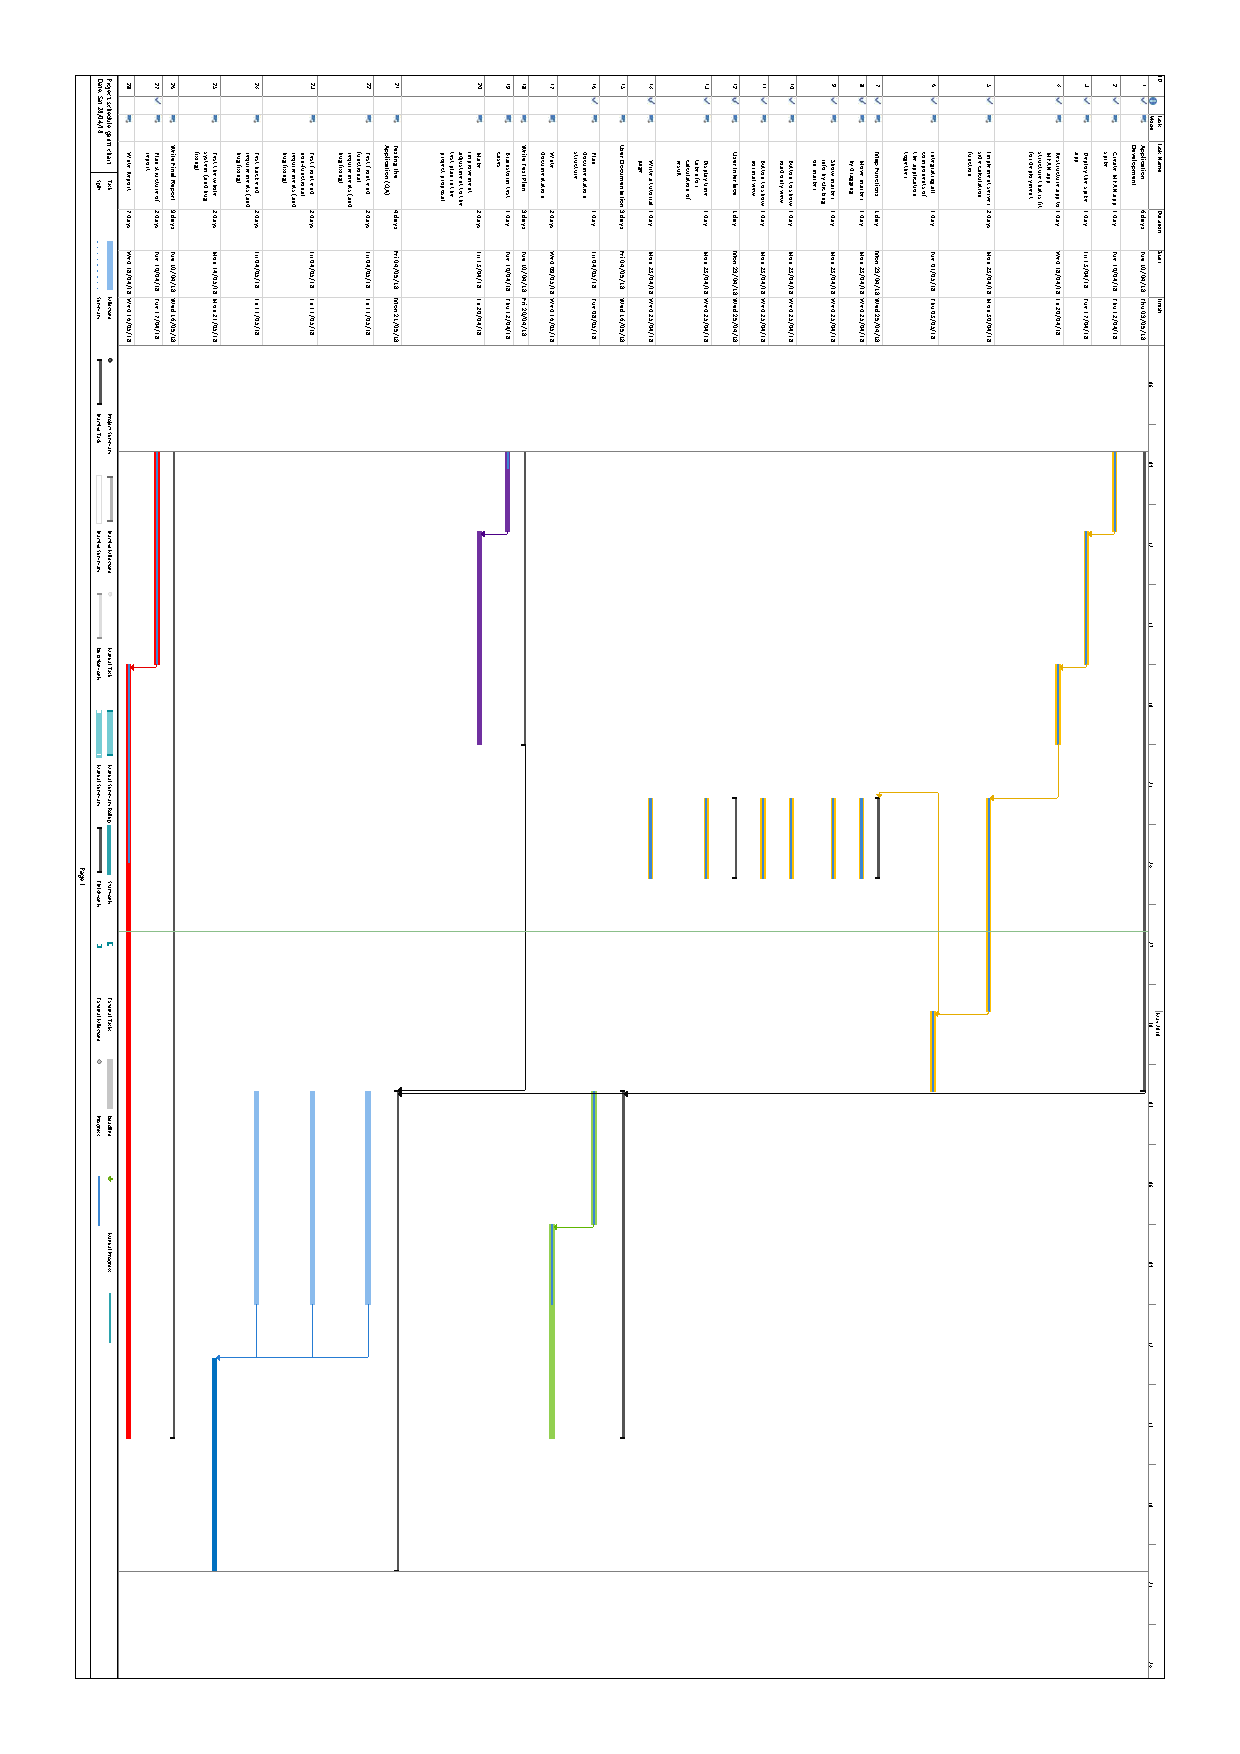
\includepdf[pages={1}]{schedule/schedule-gantt-chart-1-rotated.pdf}

As of writing the final report I'm behind schedule on my progress of the:
\begin{itemize}
	\item Final report.
	
	I'm currently behind my final report schedule progress by 2 days, but I'm expected catch up.
	
	\item Test plan
	
	I haven't started on rewriting my test plan from the project proposal yet. 
	
	\item Testing the application
	
	Although I haven't officially tested the application properly yet, I have had my application gone through usability tests and the result were good. I've also gotten criticism from the users and have made improvements to my application user interface to make my application more user friendly.
	
	\item Application documentations.
	
	I have only documented my application by 50\% so far.
	
\end{itemize}
My plan to get my project back on schedule is to first complete the final report, then complete the test report, test my application, and then document my application.
\\\\
I know that the project will be back in schedule in a week time.


%%%%%%%%%%%%%%%%%%%%%%%%%%%%%%%%%%%%%%%%%%%%%%%%%%%%%%%%%%%%%%%%%%%%%%%%

\chapter{Method}

I've used the Agile software development framework methodology in developing the project software product. For each sprint (week) I make small increments to the application. The increments are the functional and non-functional requirements. As I implement the requirements to the application I test each requirements to make sure that they are working as expected.
\\\\
The project schedule Gantt chart \hyperref[Gantt_chart:1]{figure} does not represent the Agile development life cycle I went through, but is a good basis as a list of tasks required for the project.
\\\\
I've made changes to the sequence diagram \hyperref[sequence_diagram:1]{(figure (3.2))} and software architecture diagram \hyperref[software_architecture_diagram:1]{(figure (3.3))}. I added the AJAX (Asynchronous JavaScript And XML) \cite{WEBSITE_MOZILLA_AJAX:1} technology to the diagrams. AJAX is the interface between the client HTTP call and the actual HTTP call that AJAX does asynchronously. AJAX allows the application to asynchronously calls HTTP request, which provides the advantage of having higher performance web application, because the client don't have to wait (synchronously) for the HTTP response.
\\\\
I've added AJAX to the diagrams now in the final report because I've only learned about the technology while I was developing the project's application. Developing web applications is still a new territory for me.

\section{Internal Design}
The web application will have a client-side and server-side. Angular 5 is use as the front-end client-side and Node JS Express is use as the back-end server-side. The client and server will communicates with each other through HTTP. A server is implemented in this web application so that it is properly structured and follow the separation of concerns principle. The front-end take cares of the business logic (displaying data, taking user inputs) while the back-end take cares of the calculation and processing of data.

\begin{figure}[H]
	\begin{minipage}[b]{0.4\textwidth}
		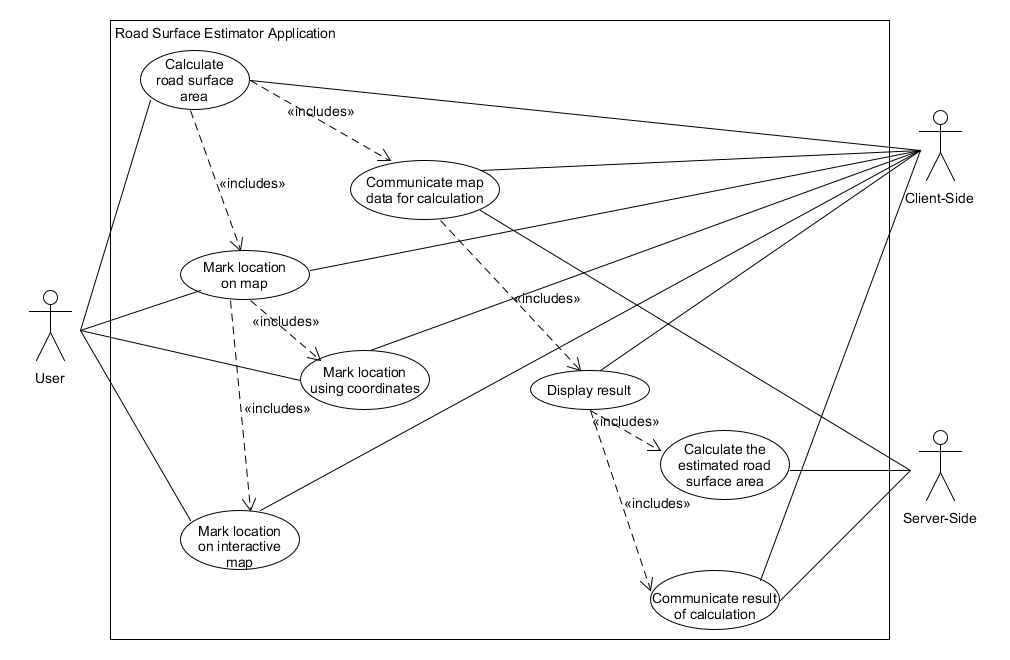
\includegraphics[scale=0.4]{use_case}
		\caption{Use Case diagram}
	\end{minipage}
\end{figure}

\begin{figure}[H]
	\begin{minipage}[b]{0.4\textwidth}
		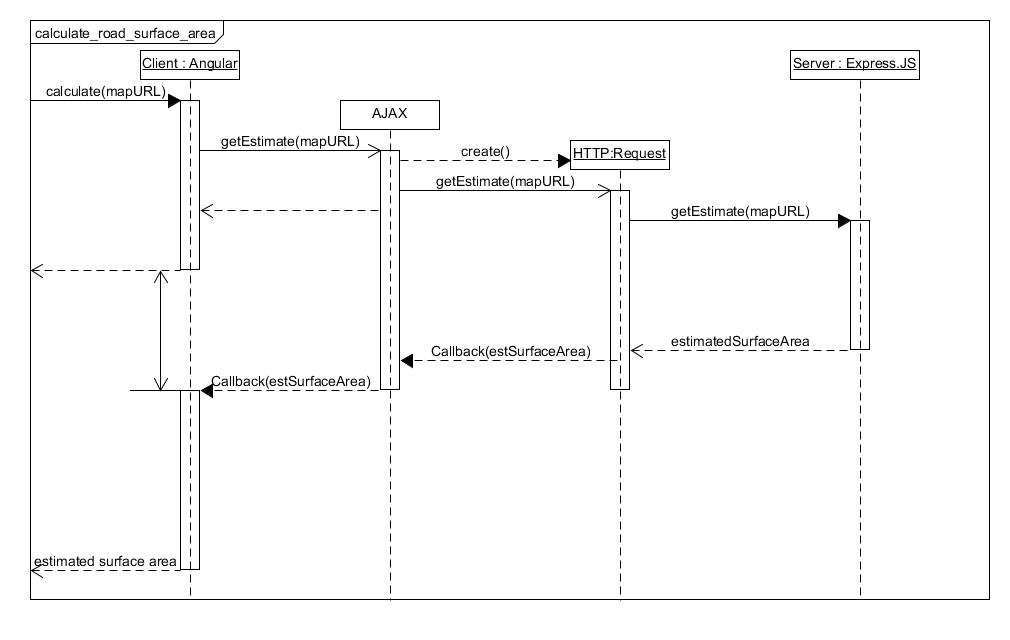
\includegraphics[scale=0.4]{squence_diagram}
		\caption{Sequence diagram}
		\label{sequence_diagram:1}
	\end{minipage}
\end{figure}

\section{Software Architecture}
The web application will use the Angular 5 web framework to implement the front-end client-side of the application. The back-end server-side will be implemented using Node JS Express, and the communications between the server and the client will be done through HTTP REST. Using the Google Maps API, the client creates a map static image URL and pass it (through HTTP) to the server for processing. The server will process the image and calculate the total surface area of roads in the map, and return the result back to the client as a response.

\begin{figure}[H]
	\begin{minipage}[b]{0.4\textwidth}
		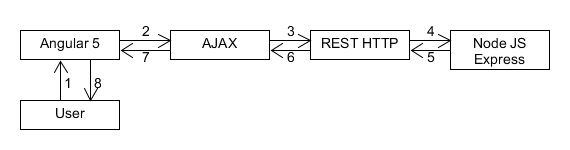
\includegraphics[scale=0.6]{software_architecture}
		\caption{Software Architecture diagram}
		\label{software_architecture_diagram:1}
	\end{minipage}
\end{figure}


\section{Algorithms}
\label{algorithm:1}

In processing the map image to calculate the estimated total surface area of roads in a nominated square kilometre, I've use get-pixels (a NodeJS package) to extract all pixels from the map image.
\\\\
With all pixels from the map I run through all pixels from the top left corner of the map to the bottom right corner of the map once. While running through each pixel the pixel is check if it is visible or not, because only road pixels in the image are visible (this was done by styling the map using the styling wizard). If the pixel is visible, it is a road pixel and a counter is incremented by 1, if the pixel is not visible then do nothing. Once all pixels have been checked, the count of road pixels are multiplied by the square metre value of each pixel, given by the formula \cite{WEBSITE_GOOGLE_GROUPS_MAPS:1}	:
\begin{center}
	$squareMetrePerPixel = metresPerPixel \times metrePerPixel$
\end{center}

\begin{center}
	$metresPerPixel = \frac{156543.03392 \times \cos(lat \times \frac{\pi}{180})}{2^{zoom}}$ 
\end{center}
where
\begin{itemize}
	\item $lat$ is the latitude is the nominated square kilometre centre coordinates latitude.
	\item $zoom$ is the current zoom level of the map.
\end{itemize}
After the multiplication the result is the estimated total surface area of all roads in the nominated square kilometre in square metres. To convert to square kilometres divide the result by 1000000.

The activity diagram (\hyperref[activity_diagram:1]{figure (3.4)}) shows the algorithm steps described above.

\begin{figure}[H]
	\label{activity_diagram:1}
	\begin{minipage}[b]{0.4\textwidth}
		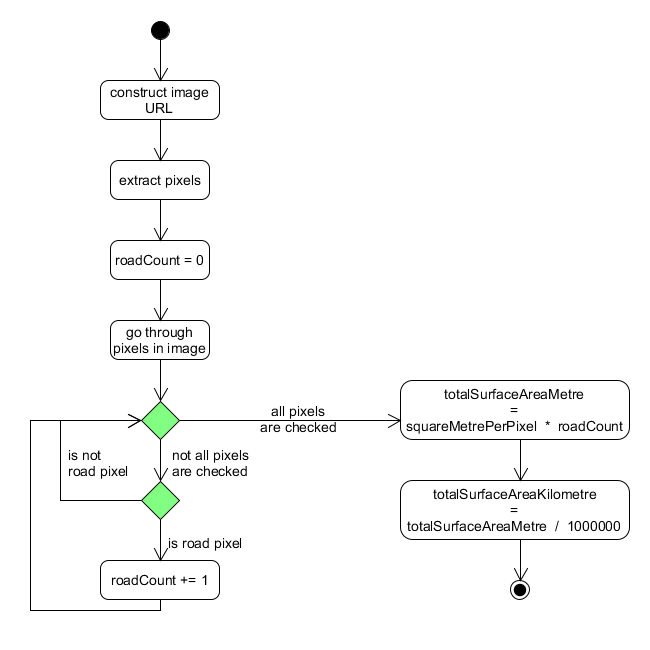
\includegraphics[scale=0.6]{algorithm.png}
		\caption{The total surface area calculation algorithm.}
	\end{minipage}
\end{figure}




%%%%%%%%%%%%%%%%%%%%%%%%%%%%%%%%%%%%%%%%%%%%%%%%%%%%%%%%%%%%%%%%%%%%%%%%

\chapter{Results}
% Analyse the OUTCOMES and QUALITY of the project.

% Talk about the requirements that were implemented in the project and their quality.
% extra features implemented in the project.
% personal opinion on what I think of the project outcome. Am I satisfied, what could have been done better.

All project requirements, both functional and non-functional are implemented in the application within the project schedule.
\\\\
There was a slight project scope creep. I introduce a new functional requirement, where the application provides a button for user to change the style of the map. This scope creep didn't affect the project schedule, since I've almost got all requirements done at that time.
\\\\
The outcome of the project was a lot better than I expected. I put a lot more emphasis on developing a good user interface than I originally intended. However, the effort I put into developing the user interface wasn't taken away from the other requirements. While working on various requirements during the project life, I continuously check the project's Gantt chart to see where I'm at in the project schedule. By checking the project schedule I remind myself where I'm at and what need to be done.
\\\\
The quality of the project is acceptable. All the requirements are implemented in the application and are satisfied.
\\\\
I'm satisfied with the outcome of the project, however I believe I could have done more with the user interface. I thought that the interface seems a little too static and needed some animations to make user experience better and more fun to use the application.

\section{Externally Observable Features}
% input, output.

% user interaction with maps
% buttons
% form inputs
The three types of input in the application are:
\begin{itemize}
	\item Google Maps
	\item Buttons
	\item Form Inputs
\end{itemize}
\underline{\textbf{Google Maps}}
\\\\
User can interact with the Google Maps using their mouse pointer and the scroll wheel. On mobile device, user interact using their fingers.
\begin{itemize}
	\item Computer Internet Browser
	\begin{itemize}
		\item click on the map to move set marker at clicked coordinates.
		\item click on marker to bring up marker info. The info is the marker's coordinates on the map.
		\item click and hold on a marker to drag it. This allow user to drag the marker around.
		\item using the scroll wheel to zoom. On the computer internet browser user must also hold "control/command" on their keyboard while scrolling wheeling to zoom.
		\item user can click and hold on the map to move the map around.
	\end{itemize}
	\item Mobile Device Internet Browser
	\begin{itemize}
		\item touch the map to move the marker to new place.
		\item touch the marker on the map to show marker coordinates info.
		\item touch and drag fingers on a marker. This action drag the marker across the map with the finger.
		\item using two fingers and making a pinching and un-pinching motion, the user can zoom the map out and in, respectively.
		\item using two fingers and dragging them across the map will move the map around.
	\end{itemize}
\end{itemize}
\underline{\textbf{Buttons}}
\\\\
The button inputs are:
\begin{itemize}
	\item a button that change map view type, showing the map in either roadView or satelliteView.
	\item a button that change map style, changing the style between the default style and a style which shows only the roads.
	\item a button that shows the calculation results and the elapsed time.
\end{itemize}
There are other input buttons such as the navigation bar links, the links in the footer, and images with links on them.
\\\\
\underline{\textbf{Form Inputs}}
There is a form with 2 input fields in the application. The input fields takes input value of type number. The input represents the latitude and longitude coordinates of the marker on the map.
\\\\
The only output from this application is the result of the calculation and the elapsed time of the calculation on the server. The result shows the surface area of roads in $km^2$ in the 1 $km^2$ area around the marker coordinates. The elapsed time shows the elapsed time of the calculation in seconds ($s$).

\section{Performance}
\label{performance:1}
% include time and space performance characteristics of your software as well as estimated complexities (including real-world processing time, storage space, bandwidth, etc.)

% elapsed time for server calculation
% elapsed time for overall calculation (time of server calculation + network communication time)

% Complexity is O(n). run through the pixel array once.

The complexity of the road surface area calculation is O$(n)$. The algorithm runs through the pixels array once, and does the area calculation afterwards. The algorithm is describe in the \hyperref[algorithm:1]{\textit{algorithm chapter}}.
\\\\
The performance result I've chosen to record are of the web application hosted Heroku \cite{WEBSITE_HEROKU:1} and accessed via the internet on Google Chrome \cite{WEBSITE_GOOGLE_CHROME:1} internet browser. I've chosen the remotely hosted version over a locally hosted version, because I wanted to test the application in a real world situation. The user would most likely use the application provided over the internet rather than locally installing the application and using. It's far easier to use it over the internet, since user only have to go to the application URL address in the internet browser. Also the performance of the web application calculation algorithm function is affected by the specifications (e.g. CPU, RAM) of the computer it is run on.
\\\\
\hyperref[thailand_data_graph:1]{Figure (4.1)} and \hyperref[melbourne_data_graph:1]{figure (4.2)} shows a line graph of the elapsed time of the calculation versus the total surface area of the roads. The result shows that there's a slight increase in elapsed time as the surface area increases. Generally the server calculation elapsed time is under the 0.25 seconds mark, and the overall calculation plus the network communication elapsed time is under 0.5 seconds.
\\\\
The \hyperref[thailand_data:1]{Thailand Data table} shows the data points for the \hyperref[thailand_data_graph:1]{Figure (4.1)} line graph and the \hyperref[melbourne_data:1]{Melbourne Data table} shows the data points for the \hyperref[melbourne_data_graph:1]{figure (4.2)} line graph. Summing up the both server time and overall time, then dividing by the number of data points result in the mean average:
\begin{itemize}
	\item Thailand Data:
	
	Server time mean average: 0.1818 seconds
	
	Overall time mean average: 0.4881 seconds
	
	\item Melbourne Data:
	
	Server time mean average: 0.192 seconds
	
	Overall time mean average: 0.6201 seconds
\end{itemize}
There were outliers in the data. The outliers are DT9, DM6, and DM8. These outlier shows the overall time being above 1 seconds, while the server time stays relatively low in comparison. My hypothesis for the occurrence of the outliers is that the Heroku server which I've hosted the application on or the internet browser that I'm using is affecting the network communication time. I've also notice that the these outlier occurs when the internet browser is idle for more than 60 seconds.
\\\\
\hyperref[thailand_data_no_outliers_graph:1]{Figure (4.3)} and \hyperref[melbourne_data_no_outliers_graph:1]{Figure (4.4)} shows line graphs of the performance data without the outliers. With no outliers, the graphs suggest that there's a correlation between the surface area and the calculation time. As the road surface area increase, so does the calculation time. My hypothesis for this correlation is that the calculation involve multiplication of each road pixels, and with higher road pixel counts (more road surface area) the multiplication required increases. The mean average of the data points with no outliers are:
\begin{itemize}
	\item Thailand Data:
	
	Server time mean average: 0.1731 seconds
	
	Overall time mean average: 0.42367 seconds
	
	\item Melbourne Data:
	
	Server time mean average: 0.176625 seconds
	
	Overall time mean average: 0.42425 seconds
\end{itemize}
Without the outliers the mean averages are lower.

\begin{figure}[H]
	\begin{minipage}[b]{0.4\textwidth}
		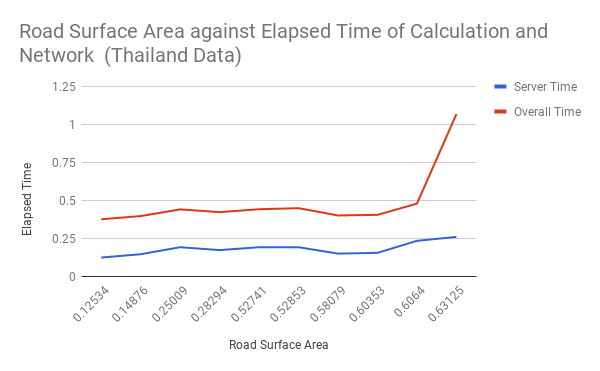
\includegraphics[scale=0.6]{thailand_data.png}
		\caption{Road Surface Area against Elapsed Time of Calculation and Network (Thailand Coordinates)}
		\label{thailand_data_graph:1}
	\end{minipage}
\end{figure}
\begin{figure}[H]
	\begin{minipage}[b]{0.4\textwidth}
		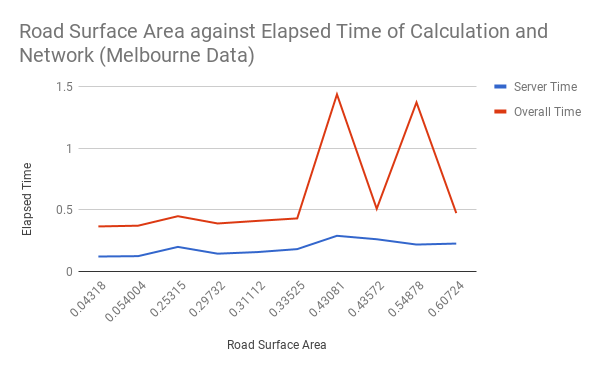
\includegraphics[scale=0.6]{melbourne_data.png}
		\caption{Road Surface Area against Elapsed Time of Calculation and Network (Melbourne Coordinates)}
		\label{melbourne_data_graph:1}
	\end{minipage}
\end{figure}

\addvbuffer[12pt 8pt]{
	\label{thailand_data:1}
	\begin{tabular}{ |p{1cm}||p{2cm}|p{2cm}|p{2cm}|p{2cm}|p{2cm}| }
		\hline
		\multicolumn{6}{|c|}{\textbf{Thailand Data}} \\
		\hline
		\textbf{ID} & \textbf{Latitude} & \textbf{Longitude} & \textbf{Result} & \textbf{Server Time} & \textbf{Overall Time} \\
		\hline
		DT0 & 13.91105564 & 100.4813004 & 0.12534 & 0.124 & 0.376 \\
		\hline
		DT1 & 13.69002205 & 100.7501221 & 0.14876 & 0.146 & 0.397 \\
		\hline
		DT2 & 13.6788381 & 100.5640411 & 0.25009 & 0.192 & 0.441 \\
		\hline
		DT3 & 13.69017971 & 100.5779457 & 0.28294 & 0.173 & 0.423 \\
		\hline
		DT4 & 13.79003496 & 100.7247162 & 0.52741 & 0.192 & 0.442 \\
		\hline
		DT5 & 13.71252776 & 100.6244659 & 0.52853 & 0.192 & 0.449 \\
		\hline
		DT6 & 13.71266717 & 100.6443787 & 0.58079 & 0.15 & 0.401 \\
		\hline
		DT7 & 13.70065954 & 100.6938171 & 0.60353 & 0.155 & 0.405 \\
		\hline
		DT8 & 13.74535151 & 100.5509949 & 0.6064 & 0.234 & 0.479 \\
		\hline
		DT9 & 13.76135851 & 100.5976868 & 0.63125 & 0.26 & 1.068 \\
		\hline
\end{tabular}}
\vspace{3mm}
\addvbuffer[12pt 8pt]{
	\label{melbourne_data:1}
	\begin{tabular}{ |p{1cm}||p{2.5cm}|p{2cm}|p{2cm}|p{2cm}|p{2cm}| }
		\hline
		\multicolumn{6}{|c|}{\textbf{Melbourne Data}} \\
		\hline
		\textbf{ID} & \textbf{Latitude} & \textbf{Longitude} & \textbf{Result} & \textbf{Server Time} & \textbf{Overall Time} \\
		\hline
		DM0 & -37.94177554 & 145.2890396 & 0.04318 & 0.121 & 0.365 \\
		\hline
		DM1 & -37.89789987 & 145.3683472 & 0.054004 & 0.124 & 0.371 \\
		\hline
		DM2 & -37.88183827 & 145.0365277 & 0.25315 & 0.199 & 0.448 \\
		\hline
		DM3 & -37.86298759 & 145.2200317 & 0.29732 & 0.144 & 0.389 \\
		\hline
		DM4 & -37.85496375 & 145.0688001 & 0.31112 & 0.157 & 0.41 \\
		\hline
		DM5 & -37.88508993 & 145.004942 & 0.33525 & 0.181 & 0.43 \\
		\hline
		DM6 & -37.81249633 & 144.9469185 & 0.43081 & 0.289 & 1.436 \\
		\hline
		DM7 & -37.84321388 & 144.9910375 & 0.43572 & 0.261 & 0.508 \\
		\hline
		DM8 & -37.81379155 & 144.9520703 & 0.54878 & 0.218 & 1.371 \\
		\hline
		DM9 & -37.8283008 & 144.9654599 & 0.60724 & 0.226 & 0.473 \\
		\hline
\end{tabular}}
\begin{figure}[H]
	\begin{minipage}[b]{0.4\textwidth}
		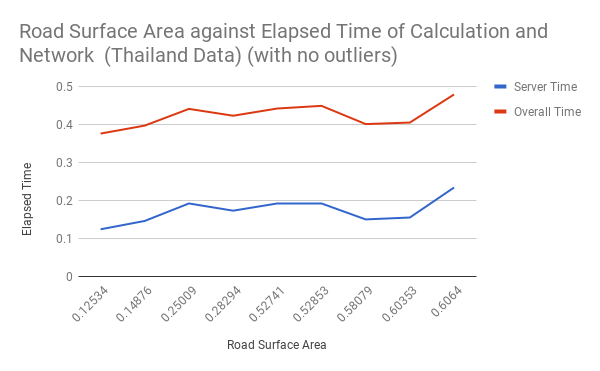
\includegraphics[scale=0.6]{thailand_data_no_outliers.png}
		\caption{Road Surface Area against Elapsed Time of Calculation and Network (Thailand Coordinates) (No Outliers)}
		\label{thailand_data_no_outliers_graph:1}
	\end{minipage}
\end{figure}
\begin{figure}[H]
	\begin{minipage}[b]{0.4\textwidth}
		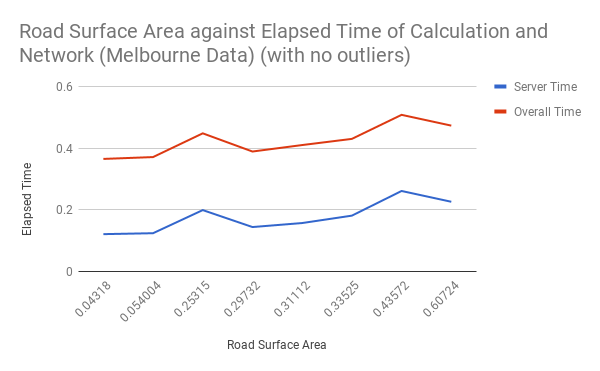
\includegraphics[scale=0.6]{melbourne_data_no_outliers.png}
		\caption{Road Surface Area against Elapsed Time of Calculation and Network (Melbourne Coordinates) (No Outliers)}
		\label{melbourne_data_no_outliers_graph:1}
	\end{minipage}
\end{figure}

%%%%%%%%%%%%%%%%%%%%%%%%%%%%%%%%%%%%%%%%%%%%%%%%%%%%%%%%%%%%%%%%%%%%%%%%

\chapter{Analysis \& Discussion}
% Analyse the statics and outputs.

% If you don’t have any idea how this kind of research might be reported, look at a few research articles in the journal JASSS: http://jasss.soc.surrey.ac.uk/JASSS.html

% The result is only an estimated. The road style in which I apply to the map to only shows the roads also shows footpath in parks, walk way on bridges

The result of the calculation for the total road surface area is only an estimate. For classifying the road pixel in the map, I've styled the map so that only the roads are visible. However, through closer investigation I've found that the map also shows walking pathway through parks and bridges as roads, and when the level of zoom is high enough (zoom in closer) some building layouts are shown. I've gone through the styling wizard \cite{WEBSITE_GOOGLE_MAPS_API_STYLING_WIZARD:1} options again to make sure that all buildings are hidden and not shown and I've confirm that all options are correct, but the same building layout are still shown.
\\\\
However, after having gone through the server side code where it constructs the image URL, I've found that the building layouts are not shown because the zoom level is too low for it to be shown. Walking pathway through parks and bridges are still shown though.
\\\\
The road surface area result is accurate enough because of the low amount of non-roads objects (walkway) in the map. Provided also that the user of this application should understand that it's an estimated and not an exact value. User can, if they choose to, prepare the exact amount of materials required for surfacing roads. The roads are already classified with a small amount of area being walkways, therefore there should be a small amount of excess material left over. This excess of material should be a small amount, because of the small surface area walkways contributes to the total estimated amount.

%%%%%%%%%%%%%%%%%%%%%%%%%%%%%%%%%%%%%%%%%%%%%%%%%%%%%%%%%%%%%%%%%%%%%%%%

\chapter{Future Work}
% Include also any possible future research that might emanate from the project.
%Google recent change for Google maps (Google Platform)

%Improve estimated result accuracy.

%Add more features to help user use the application more easily.
%- better ui for mobile and desktop (separate ui?)
%- progressive web application
%- show 1 square km around marker
%- show automatic result as marker changes (network speed consideration?)
%- graph the result (elapsed time against surface area)

%Use a software development tool chain (DevOps) to help developing the application easier and more efficient.

In future iteration of the program I would like to:
\begin{itemize}
	\item Increase the accuracy of the road surface area result.
	\item Make changes to the user interface so that it is more suitable for both computer and mobile device.
	\item Convert the application to a progressive web app (PWA) \cite{WEBSITE_GOOGLE_PWA:1}.
	\item Shows a 1 $km^2$ square border line around the map marker.
	\item Shows the result automatically as the marker coordinates changes.
	\item Keeps record of the result data and visualise it.
	\item Implement better Development Operations (DevOps).
\end{itemize}
\underline{\textbf{Increase result accuracy}}
\\
To increase the result accuracy I might have to find a way to get remove the walkways from the road classifications. To go about doing this I will research the Google Maps API maps object further to see if I could find out what kind of object the walkways are and if I can hide it.
\\\\
\underline{\textbf{UI being more suitable for computer and mobile devices view}}
\\
I considering implementing a feature that checks what device the user is on and display an appropriate version of the application to the user so that the view is optimise for the device and screen size.
\\\\
\underline{\textbf{Convert application to PWA}}
\\
My application stack is a \textit{MEAN} without the \textit{M} (MongoDB, use as database). I've had a look at web tutorials and videos guide on converting application to PWA. I'm considering creating a branch of the application and experimenting with converting the application to a PWA.
\\\\
\underline{\textbf{1 $km^2$ square borderline}}
\\
I've seen other students in class implemented this feature in their application, and I've asked them about it. I was given a brief explanation on how to implemented it. The problem that I foresee for implementing the Google Maps geometry is that the Google Maps API I'm currently using is a library Angular 5 wrapper of Google Maps \cite{WEBSITE_AGM:1}. I'll have to find out if drawing geometry can be done with the wrapper.
\\\\
\underline{\textbf{Shows result as marker moves}}
\\
This feature is easy to implement. I can attach a event listener to the dragging event of the marker and call a calculation each time the marker is move. However, the problem with continuously making a calculation as the marker moves is the calculation elapsed time. As shown above in the \hyperref[performance:1]{performance chapter}, the overall elapsed time for calculation and network communication on mean average is around under 0.5 seconds. The calculation elapsed time might be a problem, affecting the user experience. Experiments need to be done having users test out the feature and see if its too slow for their liking.
\\\\
\underline{\textbf{Visualise the result data}}
\\
Implement a local storage on the client side or MongoDB in the back end server. Storing user calculation results there and visualise it using D3 \cite{WEBSITE_D3:1} or some other data visualisation libraries.
\\\\
\underline{\textbf{Better DevOps}}
\\
Implement a tool chain in the application development operation. Implement testing tools such as Travis CI for testing the application and Docker for packaging the application.
\\\\
Another future work of the project I would like to discuss is the recently introduced Google Maps Platform on 02$\backslash$05$\backslash$2018. The new platform combines the various Maps API into products: "We’re simplifying our 18 individual APIs into three core products—Maps, Routes and Places, to make it easier for you to find, explore and add new features to your apps and sites. And, these new updates will work with your existing code—no changes required." \cite{WEBSITE_GOOGLE_BLOG:1}. Note that the last sentence says the existing code will still work as intended, so there's no change needed for the project.
\\\\
The new platform also introduce a new pricing plan, where instead of a free tier, the developer get a \$200 of free usage each month: "With this new plan, developers will receive the first \$200 of monthly usage for free.", "With this new pricing plan you’ll pay only for the services you use each month with no annual, up-front commitments, termination fees or usage limits." \cite{WEBSITE_GOOGLE_BLOG:1}.
\\\\
However, one should also take into consideration the maximum limits of loads available for the free tier (free \$200 monthly). The maximum amount of loads for Dynamic Maps, which is the JavaScript Maps API is 28,000 loads for month \cite{WEBSITE_GOOGLE_BLOG:2}. This maximum limitation of loads should be taken into consideration if the application in this project is to be use by large user groups, since a limit might be reach.
\\\\
Further study of the new Google Maps Platform is needed to gain more insight into the change.


%%%%%%%%%%%%%%%%%%%%%%%%%%%%%%%%%%%%%%%%%%%%%%%%%%%%%%%%%%%%%%%%%%%%%%%%

\chapter{Conclusion}

In conclusion I thought the project went very well and even exceeded my expectation. I've added a lot more features (requirements) than the specified requirements in the project proposal. The project was completed a head of schedule by 2 weeks. Being so ahead of schedule, perhaps more features from the future work section could be implemented.
\\\\
Developing the application have been a good experience and a good opportunity to implement what I've learned during my degree course and what I've learned on my own. I've applied what I've learn in project management unit with this project, creating concise documentations and sticking to schedule.
\\\\
I know that there are a lot more that I can do to the project to improve it. This is a good thing, since one should always strive for betterment and improvement in one's self and in one's work. I will continue to work on the project and make improvement to it.


%%%%%%%%%%%%%%%%%%%%%%%%%%%%%%%%%%%%%%%%%%%%%%%%%%%%%%%%%%%%%%%%%%%%%%%%

\chapter{References}
% Organise the bibliography alphabetically by first-author surname or by order of appearance in the article.

\bibliography{reference/reference}
\bibliographystyle{apalike}

%%%%%%%%%%%%%%%%%%%%%%%%%%%%%%%%%%%%%%%%%%%%%%%%%%%%%%%%%%%%%%%%%%%%%%%%

\chapter{Appendices}

\section{Production and Deployment}
% Detail instructios to run/install/compile your software, with complete instructions/screenshots. Include all information such as dependencies, platform, etc.
Legend:
\begin{itemize}
	\item command are written in \textbf{bold} style.
	\item file and file directory are written in \textit{italic} style.
\end{itemize}
Below are the instructions on how to run the web application locally on the host computer.
\\\\
Install Node.js from \url{https://nodejs.org/en/download/}.
\\\\
Install angular cli tool globally on the system using npm package manager (this command may require administrative privilege, if so put \textbf{sudo} in front of the command when using Linux system):
\\
\textbf{npm install -g @angular/cli}
\\
or (if require admin privilege on Linux system)
\\
\textbf{sudo npm install -g @angular/cli}
\\\\
To install the application run \textbf{npm install} at the root directory of the application. This install all node module dependencies required for running the application. All dependencies for the application can be found in the \textit{package.json} file at the root directory of the application.
\\\\
The application requires the client server and back end server to be run at the same time.
\\\\
Run \textbf{node server.js} for a backend Express.JS server API.
\\\\
Run \textbf{ng serve} for a client server. Navigate to \textit{http://localhost:4200/} to access the web application.


\section{User Interface}
% How to run the software.
% Detail clearly the interface(s) to the Web-based project.

The web application consist of a set of web pages, a navigation bar at the top of the screen (\hyperref[navigation:1]{figure (9.1)}), and a footer at the bottom of the screen (\hyperref[footer:1]{figure (9.2)}).
\begin{figure}[H]
	\begin{minipage}[b]{0.4\textwidth}
		\label{navigation:1}
		
\includegraphics[scale=0.6]{navigation.png}
		\caption{The navigation bar at the top of the page.}
	\end{minipage}
\end{figure}
The navigation and footer can be use to explore the pages of the application.
\begin{figure}[H]
	\label{footer:1}
	\begin{minipage}[b]{0.4\textwidth}
		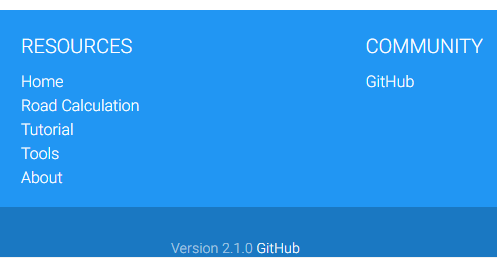
\includegraphics[scale=0.6]{footer.png}
		\caption{The footer at the bottom of the page.}
	\end{minipage}
\end{figure}
A page in the application is dedicated as a tutorial to the usage of the road surface area calculation function (\hyperref[tutorial:1]{figure (9.3)}). The tutorial include images and descriptions to describe the usage.
\begin{figure}[H]
	\label{tutorial:1}
	\begin{minipage}[b]{0.4\textwidth}
		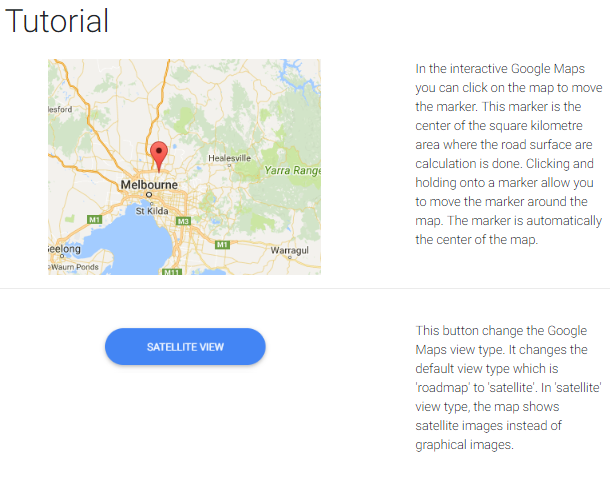
\includegraphics[scale=0.6]{tutorial.png}
		\caption{The tutorial page.}
	\end{minipage}
\end{figure}

\section{Externally Available Functions}
% Debuggin tools, auxilliary/helper function, bonus features.
There are currently no external functions available for the server. I didn't consider adding any, because I've not implemented any before and because I wasn't thinking about it. Also the application is only of a small scale and won't likely benefit much from any external functions.

\section{Internal Testing Procedures}
% Cross-references to Test Report.
I haven't implemented any internal testing procedures for the application. I've tested the application using primitive methods such as manually testing the functions and console logging variables to check the state of the application. The tests are described in the test report \cite{DOCUMENT_TEST_REPORT:1}.

%%%%%%%%%%%%%%%%%%%%%%%%%%%%%%%%%%%%%%%%%%%%%%%%%%%%%%%%%%%%%%%%%%%%%%%%

\end{document}